% title: Fully connected network (MLP)
% description: Multilayer perceptron with input, hidden and output layers of neurons, dense connections, an ellipsis for wide layers, and layer labels with sizes and activations. Change \layers to resize it.
\documentclass[tikz,border=10pt]{standalone}
\usepackage{amsmath,amssymb}
\usetikzlibrary{arrows.meta,positioning,calc}

\definecolor{inp}{HTML}{C6E5F7}
\definecolor{hid}{HTML}{FCE0BE}
\definecolor{outc}{HTML}{CBEACF}

\tikzset{
  every node/.style={font=\sffamily\small},
  neuron/.style={circle, draw, line width=0.6pt, minimum size=7mm, inner sep=0pt},
  edge/.style={line width=0.3pt, draw=black!45},
  layerlabel/.style={align=center, font=\sffamily\small},
}

% Layers: index / visible neurons / color / label / math label prefix
\newcommand{\layers}{1/4/inp/{Input\\$x\in\mathbb{R}^{784}$}/x, 2/5/hid/{Hidden 1\\$512$, ReLU}/h, 3/5/hid/{Hidden 2\\$256$, ReLU}/g, 4/3/outc/{Output\\$10$, softmax}/y}

\begin{document}
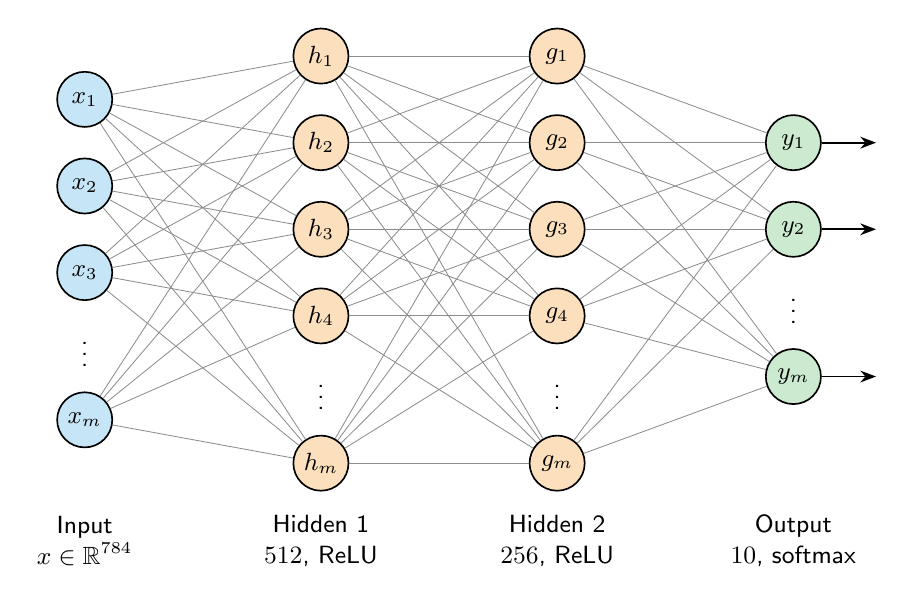
\begin{tikzpicture}[x=30mm, y=11mm]

\foreach \l/\n/\c/\lbl/\sym in \layers {
  \foreach \i in {1,...,\n} {
    \pgfmathsetmacro{\yy}{(\n+1)/2-\i-(\i==\n ? 0.7 : 0)}
    \ifnum\i=\n
      \node[neuron, fill=\c] (n\l-\i) at (\l,\yy) {$\sym_{m}$};
    \else
      \node[neuron, fill=\c] (n\l-\i) at (\l,\yy) {$\sym_{\i}$};
    \fi
  }
  \node[layerlabel] at (\l,-3.6) {\lbl};
}

% Ellipsis between the last two neurons of each layer.
\foreach \l/\n/\c/\lbl/\sym in \layers {
  \pgfmathtruncatemacro{\prev}{\n-1}
  \node at ($(n\l-\prev)!0.5!(n\l-\n)$) {$\vdots$};
}

% Dense connections between consecutive layers.
\foreach \l/\n in {1/4, 2/5, 3/5} {
  \pgfmathtruncatemacro{\next}{\l+1}
  \pgfmathtruncatemacro{\m}{\next==4 ? 3 : 5}
  \foreach \i in {1,...,\n} {
    \foreach \j in {1,...,\m} {
      \draw[edge] (n\l-\i) -- (n\next-\j);
    }
  }
}

\foreach \j in {1,...,3} {
  \draw[-{Stealth[length=2mm]}, line width=0.6pt] (n4-\j) -- ++(0.35,0);
}

\end{tikzpicture}
\end{document}
